%Obviously, the waiting cost of synchronous aggregation is sometime harmful, So we proposed using asynchronous aggregation to reduce the coordination.
%In this section, we first formally define asynchronous aggregation and introduce accumulated recursive aggregation program. We then propose the sufficient conditions for returning correct results by analyzing the aggregate/non-aggregate operations.And then we propose a conversion technology for some unsatisfied algorithm.
%In this section, we propose the foundations of automatic asynchronous aggregation.

\subsection{Asynchronous Aggregation}
\label{sec:async:async}

The recursive program in Equation (\ref{eq:recursive2}) is defined with synchronous aggregation. In the $k$th iteration, suppose the aggregate operation $g_{p}^k()$ associated with key $p$ will be applied on the subsets $\{Y_{p,1}^k,Y_{p,2}^k,\ldots,Y_{p,m}^k\}$. The synchronous aggregate operation has to wait for all its inputs to perform aggregation $g_{p}^k(Y_{p,1}^k,Y_{p,2}^k,\ldots,Y_{p,m}^k)$ before starting the $(k+1)$th round of $F$ operations. Correspondingly, we define asynchronous aggregation as follows.
%on all subsets $\{Y_{k_p 1}^k,Y_{k_p2}^k,\ldots,Y_{k_pm}^k\}$ have to be completed before the next $G()$ operation starts. %The $g()$ operation has to be applied on the whole set $X^k$.


\begin{comment}
\begin{definition}
	%wqg
	%\label{def:asyncaggre}
	(\textbf{Asynchronous Aggregation}) In a recursive program, for an aggregation g() we assume that the input  $x$  is partitioned into $m$ disjoint subsets by the recursion,and denote as $x^{r_i}$ i.e., $x=\{x^{r_1},x^{r_2},\ldots,x^{r_m}\}$, and $\forall i,j, x^{r_i}\cap x^{r_j}=\emptyset$. Asynchronous aggregation is to aggregate multiple subsets from different recursions,i.e.$g(x)=g(x^{r_1},x^{r_2},\ldots,x^{r_m})$.

For a group-by aggregate operation. the inputs can be partition by their keys i.e.$X=\{X_{k_0},X_{k_1}\ldots,X_{k_n}\}$, or by the iterations i.e.$X=\{X^{r_0},X^{r_1}\ldots,X^{r_m}\}$ in which $X^{r_i}$ denote the subset in its $i$th recursion from all the keys, i.e.$X^{r_i}=\{X_{k_0}^i\cup X_{k_1}^i\cup ....\cup X_{k_n}\}$.Supposed the inputs $X$ come from $m$ different recursion, The asynchronous group-by  aggregation is defined as $G(X)=G(X^{r_0},X^{r_1}\ldots X^{r_m})$
\end{definition}

From the definition of recursive aggregation as shown in Equation (\ref{eq:recursive2}), $X^{k+1}$ is resulted from $Y^k$, and $Y^k$ is resulted from $X^k$. $X^{k+1}$ does not exist before applying $g()$ on the complete set of $X^k$. Thus, the asynchronous aggregation $g(\ldots X_i^k\cup X_j^{k+1} \ldots)$ is only possible after the $j$th subset of $X^{k+1}$ is obtained. In other words, $X^{k+1}$ is a \emph{replacement} of $X^k$ and is closer to the final result. The asynchronous aggregation of $X^{k+1}$ and $X^k$ may result in a wrong result since $X^k$ is a replaced result which is not supposed to be aggregated.
\end{comment}

\begin{definition}
	\label{def:asyncaggre}
	(\textbf{Asynchronous Aggregation}) In a recursive program, we assume that the input set $Y_{p}^k$ for key $p$ from the $k$th recursion is partitioned into $m$ disjoint subsets, i.e., $Y_{p}^k=\{Y_{p,1}^k,Y_{p,2}^k,\ldots,Y_{p,m}^k\}$, and $\forall i,j, Y_{p,i}^k\cap Y_{p,j}^k=\emptyset$. The asynchronous aggregation is to aggregate multiple subsets from different recursions, i.e., $g(\ldots Y_{p,i}^k\cup Y_{p,j}^{l}\ldots)$ where $k\neq l$.
	% $Y_j^l=\cup_{k_i\subset K}Y_{k_i}^l$
	%{\color{red} does \ldots necessary, please make a dicision}
\end{definition}

Since the group-by aggregation is composed of many key-specified aggregations, the asynchronous group-by aggregation can be similarly defined as $G(\ldots Y_{i}^k\cup Y_{j}^{l}\ldots)$ where $k\neq l$ and $Y_i^k$ is the $i$th kv-pairs subset from the $k$th recursion.

% the whole set can be partitioned into $m$ disjoint subsets,i.e. $Y^k=\{Y_{ 1}^k,Y_{2}^k,\ldots,Y_{m}^k\}$  and $\forall i,j, Y_{i}^k\cap Y_{j}^k=\emptyset$. Asynchronous group by aggregation is to aggregate multiple subsets from different recursions, i.e., $G(\ldots Y_{i}^k\ldots\cup Y_{j}^{l}\ldots)$ where $k\neq l$.

From the definition of recursive aggregation in Equation (\ref{eq:recursive2}), $X^{k+1}$ is resulted from $Y^k$, and $Y^k$ is resulted from $X^k$. $X^{k+1}$ does not exist before applying $G\circ F()$ on the complete set of $X^k$. Thus, the asynchronous aggregation $g(X_i^k\cup X_j^{k+1})$ is only possible after $X^{k+1}$ is obtained. In other words, $X^{k+1}$ is a \emph{replacement} of $X^k$. The asynchronous aggregation of $X^{k+1}$ and $X^k$ may result in a wrong result since $X^k$ should be replaced which is not supposed to be aggregated.

\section{Asynchronize Recursive Aggregation}
\subsection{Accumulated Recursive Aggregation}
\label{sec:async:accrec}

{To support asynchronous processing and intergrate the advantage of semi-naive evaluation, we proposed a special form of recursive aggregation  \textbf{accumulative recursive aggregation}.
	\begin{figure}[t]
		\vspace{-0.1in}
		\centerline{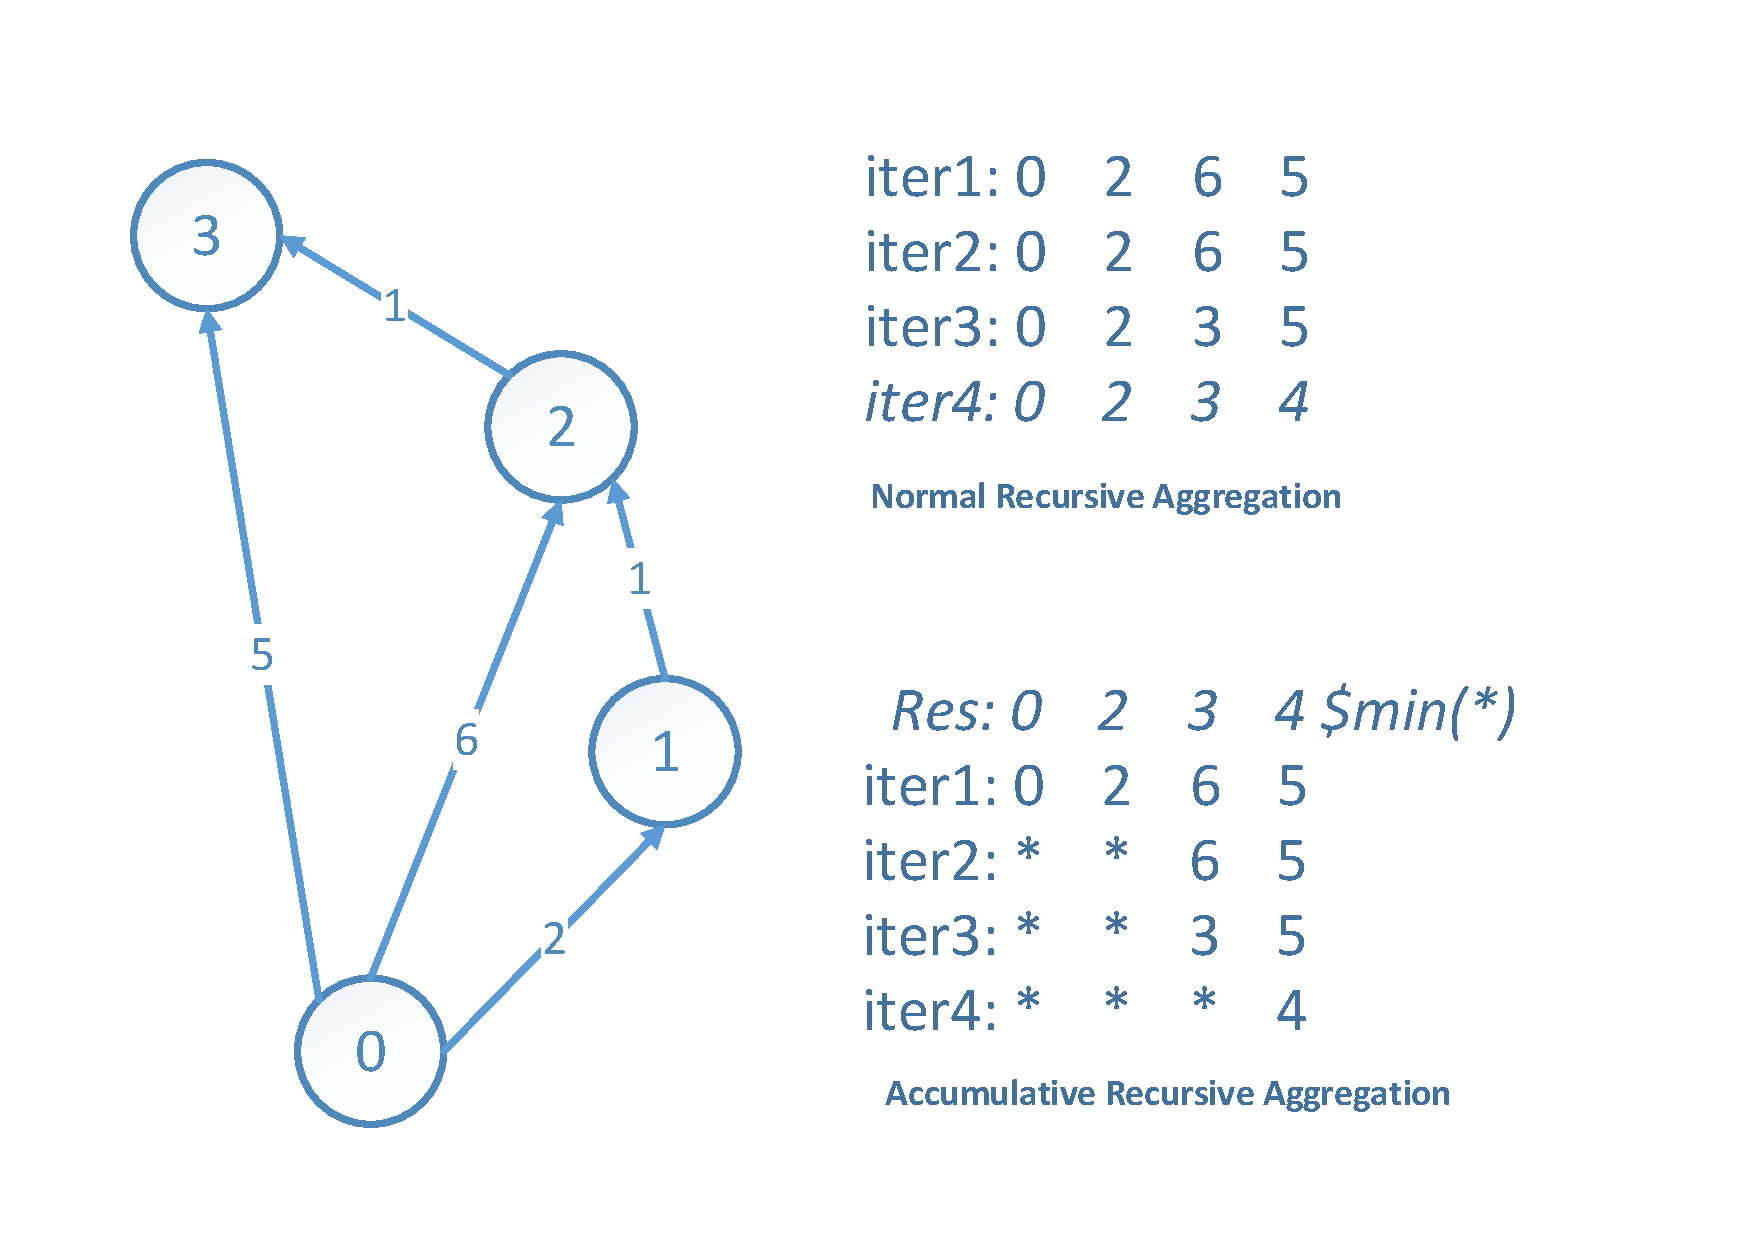
\includegraphics[width=3in]{fig/sssp-example.pdf}}
		\caption{An accumulative recursive example with SSSP algorithm}
		\vspace{-0.1in}
		\label{fig:arasssp}
	\end{figure}
	
	
We observed that some of the Recursive aggregation has the potential to be evaluated incrementally, when monotonic conditions are satisfied. i.e., The result of the previous recursion needs to involved in the next recursion. Take SSSP as example, the $\$min$ operation takes both newly generated paths and the current minimum distance as input to find the minimum distance. We find that these program can be rewrite as accumulative recursive aggregation forms that has the potential to asynchronouly processing e.q., figure \ref{fig:arasssp}. Hence we gives the definition and constraint of accumulative aggregation.


\begin{definition}
	\label{th:monotone}
	(\textbf{Accumulable}) 
	\begin{itemize}
		\item \textbf{communitive}: $G(Y_1\cup Y_2)=G(Y_2\cup Y_1)$
		\item \textbf{monotonic}: $X\subseteq F(X)$
		\item \textbf{accumulative}: $G(Y_1\cup Y_2)=G(G(Y_1)\cup Y_2)$
	\end{itemize}
	A normal recursive aggregate form is able to convert to accumulative recursive aggregations, if the aggregate operation $G$ is communitive and accumulative and non-aggregate operations $F$ is monotonic. We call it accumulable.
\end{definition}
	
	\textbf{Accumulated Recursive Aggregation.} If a normal recursive aggregation  as defined with equation (\ref{eq:recursive2}) is accumulable, and make $F\delta(X)=F(X)-X$,  the accumulated recursive aggregation form can be represented as follows.
	\begin{equation}\label{eq:accumasync}
	\begin{aligned}
	\Delta Y^{k}&= F_{\delta}(\Delta X^k)\\
	\Delta X^{k+1}&= G(\Delta Y^{k})\\
	X^{n}&=G(\cup_{i=0}^{n-1} \Delta X^{i})
	\end{aligned}
	\end{equation}
	It iteratively computing the increments by starts from $\Delta X^0=X^0$ and terminates when there is no new $\Delta X^k$ produced. And the final result is the aggregation of all intermediate results. We can easily proof that the accumulative recursive aggregation return the same result with normal recursive aggregation as equation (\ref{eq:recursive2}).
	\begin{proof}
	\label{sec:app:proof:monotonic}
	Since $\Delta Y^k=F_\Delta(\Delta X^k)$ and $\Delta X^0=X^0$.
	\small
	\begin{align}
	&G\Big(\Delta Y^0\cup F_\Delta \circ G(\Delta Y^0)\cup\ldots\cup (F_\Delta\circ G)^k(\Delta Y^0)\Big)\notag \\
	=&G\Big(G(\Delta Y^0)\cup F_\Delta\circ G(\Delta Y^0)\cup \ldots \cup (F_\Delta\circ G)^k( \Delta Y^0)\Big)\notag\\
	=&G\Big(F\circ G(\Delta Y^0)\cup (F_\Delta\circ G)^2(\Delta Y^0)\cup \ldots \cup (F_\Delta\circ G)^k(\Delta Y^0)\Big) \notag\\
	=& \ldots \notag \\
	=&G\Big((F\circ G)^k(\Delta Y^0)\Big)\notag\\
	=&(G \circ F)^{k+1}(X^0)\notag
	\end{align}
	\normalsize
	Line (2) is true because the accumulative and communitive property and line (3) is true because monotonic property, then we can obtain the final result by repeatly applying these two property, which has the same form with normal recursive aggregation.
\end{proof} 

{\color{red}
Accumulative recursive aggregation program has similar form and constraints with seminaive technology. But they are essentially different.
seminaive technology was proposed to redcuce redudant computation. While accumulative recursive aggregation aims at incrementally evaluate the original datalog program to support asynchronous processing. However, the accumulative recursive aggregation program can also be evaluated with semi-naive technology. if the previous $bag$-$monotonic$ conditions are satisfied.}

{\color{green}	
accumulative recursive aggregation program can also be evaluated with semi-naive technology, 
But not all semi-naive program can be expressed with accumulate recursive aggregates form.  % previous works proposed that some of the recursve aggregation program can be conditionally converted to incremental evaluation(using seminaive-evaluation).
Based on the previous fundation, accumulative recursive aggregation  satisfied the $bag$-$monotonic$ conditions, but there is a little more constraint.
based on these observation we summarize the correctness conditions of accumulated recursive aggregation as follow.
}


{\color{green}
Intuitively, the accumulated recursive program performs the same computation as normal recursive program, but the final result is the aggregation of all the intermediate results as shown in Equation (\ref{eq:accumasyncres}). The asynchronous aggregation becomes meaningful in accumulated recursive programs, since the final result is the \emph{aggregation} of all recursions' results but not the last recursion's result. $\Delta X^{k}$ represents the \emph{increment} from previous recursion but not a replacement of previous recursion. This implies that the accumulated recursive aggregation exhibits \textbf{monotonicity}, which has been well studied in the literature \cite{Hellerstein:2010:DIE:1860702.1860704,calm,Lam:2013:SDE:2510649.2511289,Wang:2015:AFR:2824032.2824052}. Briefly speaking, monotonicity means that we only add information, never negate or take away. However, not all recursive programs are monotonic. We have the following theorem to guide the transformation.
}
%Converting an Recursive aggregation into accumulative recursive aggregate should  

{\color{green}
Since $G$ and $F$ are group-by operations of $g$ and $f$, the group-by operations satisfy the conditions only if $g$ and $f$ satisfied the same condition for each key.In order to facilitate expression and proof,we use the group-by operation to formalize the definition and proof.We provide the formal proof.}

\begin{comment}
{\color{blue}
	\begin{itemize}
		\item \textbf{community}: $G(Y_1\cup Y_2)=G(Y_2\cup Y_1)$
		\item \textbf{associate}: $G(G(Y_1)\cup Y_2)=G(Y_1\cup G(Y_2))$
	\end{itemize}
	The associate property can be infered from accumulative property if community property satisfied.
	\begin{equation}
	\begin{aligned}
		&G(G(Y_1)\cup Y_2)=G(Y_1\cup Y_2)\\\notag
		=&G(Y_2\cup Y_1)=G(G(Y_2)\cup Y_1)\\\notag
		=&G(G(Y_2)\cup Y_1)\notag
	\end{aligned}
\end{equation}


::::::::::::::::::::::::::::::::::::

	I haven't infer the accumulative property from associate and community. But the seminaive condition socialite proposed is no longer essential(we have bag-monotonic conditions). So i am a little 
	hesitate about this place, i'd like to remove these blue statement. 
	
}
\end{comment}




The accumulative property is not only essential in theorem proof but also helpful for efficient system design. If the accumulative condition is satisfied, only the aggregation result $X^k=G(\Delta Y^{0},\ldots,\Delta Y^{k-1})$ needs to be maintained (i.e., the maintained result set size is equal to the number of unique keys) and is updated by accumulating a new $\Delta Y^{k}$, i.e., $X^{k+1}=G(Y^k \cup \Delta Y^k)$. Otherwise, the large set $\Delta \{Y^{k}\}$ needs to be maintained for every recursion $k$, which incur considerable storage cost. The accumulative property will be exploited in our system design to save a lot of maintaining cost. And also accumulative is also inportant in asynchronous conditions.

{\color{blue}
I have some disputes about these statement. It is related with the conversion conditions which can be temporarily removed:::	
	
	
There is a special case of aggregates $count$, which doesn't satisfied the accumulative property but can also write as accumulative form:
\begin{equation}
\label{eq:accumasyncres}
G^+\Big(G(\Delta Y^0)\cup G(F\circ G)(\Delta Y^0)\cup\ldots\cup G(F\circ G)^k(\Delta Y^0)\Big).
\end{equation}
in which $G^+$ is $\$sum$ operations. it can be evaluated with semi-naive technology , but hard to asynchronous.
}
%\Paragraph{Example 1: Compuiting Paths in a DAG} This algorithm (denoted as \textbf{PATHS}) counts the paths between all pairs of vertices in an acyclic graph. The number of paths between vertex $s$ and vertex $d$, $path(s,d)$, is initialized as $1$ for each edge $(s,d)$ and $0$ for others. The $f$ operation of the $k$th recursion for vertex pair $(s,d)$ takes $path^k(s,d)$ as input and outputs $path_{tmp}^k(s,d')$ if edge $(d,d')$ exists. The aggregation operation $g()$ with respect to each pair $(s,d')$ takes all $path_{tmp}^k(s,d')$ as inputs and computes $path^{k+1}(s,d')=\sum_{d'} path_{tmp}^k(s,d')+path^k(s,d')$ as the result. The computation terminates when the path numbers for all vertex pairs are not changed from previous recursion.

%\textcolor{red}{this description seems to be wrong in many parts, including some lables. I can't fix them one by one. Please make them consistent with the previous description of Example 1}
%For example,
% the paths computation (Example 1) can be executed as an accumulated recursive program. Its non-aggregate operation $f()$ on vertex pair $(s,d)$ outputs not only the tuples set $\{path_{tmp}^k(s,d')\}$ to $d$'s outgoing neighbors $d'$ but also its previous recursion's aggregation result $path^k(s,d)$. That is, $\{path_{tmp}^k(s,d')\}$ and $path^k(s,d)$ are all contained in $f(path^k(s,d))$. Hence, $X^{k}\subseteq F(X^{k})$ and the monotonic condition is satisfied. In addition, the aggregate operation $g()$ which is SUM has the accumulative condition.
%the SSSP computation (Example 2) can also be executed as an accumulated recursive program. Its non-aggregate operation $f()$ on node $i$ outputs not only the tuples set $\{\langle j,td_j^{k+1}\rangle\}$ for its outgoing neighbors $j$ but also its previous recursion's aggregation result $\langle i,d_i^k\rangle$. That is, $\{\langle i,td_i^{k+1}\rangle\}$ and $\langle i,d_i^k\rangle$ are contained in $X^{k+1}$, while $\langle i,d_i^k\rangle$ is already contained in $X^{k}$. Hence, $X^{k}\subseteq X^{k+1}$ and the monotonic condition is satisfied. In addition, the aggregate operation $g()$ which is MIN has the accumulative and commutative conditions.


\subsection{Conditions for Asynchronous Aggregation}
\label{sec:async:condition}

As discussed, asynchronous aggregation is possible in accumulated recursive programs. However, not all accumulated recursive programs with asynchronous aggregation will return the same result as that with synchronous aggregation. We demonstrate the sufficient conditions for asynchronous aggregation in the following theorem.

\begin{theorem}
	\label{th:async}
	(\textbf{Asynchronizability}) With asynchronous aggregation as described in Definition \ref{def:asyncaggre}, an accumulated recursive program will yield to the same result as with synchronous aggregation after the $F$ and $G$ operations are performed infinite times, as long as the following conditions are satisfied.
	\begin{itemize}
		\item \textbf{order independent}: $G\circ F\circ G(X)=G\circ F(X)$;
		\item \textbf{commutative}: $G(Y_1\cup Y_2)=G(Y_2\cup Y_1)$;
	\end{itemize}
\end{theorem}

By asynchronous aggregation, the partial aggregation result is immediately used by the next $F()$ operation. The order independent property implies that no matter the $F()$ operation is first applied or the $G()$ operation is first applied, the effect is the same. As long as the same number of $G()$ operations are applied on all data, the eventual aggregation result will be the same.%Due to de definition ,it is obvious that $G$and $F$ operations also satisfied order-independent and commutative properties in this condition.
Here we give the formal proof,

\begin{proof}
	\label{sec:app:proof:correct}
	In this proof, We assumed that $X$ can be divided into two disjoint subset $X_0$ and $X_1$. we exchange the subset belongs to any two  recursion, and then prove that they have the same formula with the origin form. Exchanging the subset for one time is the basic form which can generalize all the general situation by exchanging the subset from two arbitrary recursion arbitrary times under different division.
	\begin{align}
	&G(\Delta X^0\cup \ldots \cup F\circ G(\Delta X^{i}_0 \cup \Delta X^{j}_1)\cup\ F\circ G(\Delta X^{j}_0 \cup \notag\\ &\Delta X^{i}_1) \ldots\cup \Delta X^n)\tag{1} \\
	=&G( \ldots \cup G \circ F\circ G(\Delta X^{i}_0 \cup \Delta X^{{j}}_1)\cup\ G \circ F\circ G(\Delta X^{{j}}_0 \cup \notag\\ &\Delta X^{i}_1) \ldots)\tag{2} \\
	=&G( \ldots \cup G \circ F(\Delta X^{i}_0 \cup \Delta X^{{j}}_1)\cup\ G \circ F(\Delta X^{{j}}_0 \cup \Delta X^{{i}}_1) \ldots)\tag{3} \\
	=&G( \ldots \cup (G\circ F(\Delta X^{i}_0) \cup G\circ F(\Delta X^{{j}}_1))\cup\ (G \circ F(\Delta X^{{j}}_0) \notag\\ &\cup G \circ F(\Delta X^{i}_1)) \ldots )\tag{4} \\
	=&G( \ldots \cup (G\circ F(\Delta X^{i}_0) \cup G\circ F(\Delta X^{i}_1))\cup\ (G \circ F(\Delta X^{{j}}_0) \notag\\ &\cup G  \circ F(\Delta X^{{j}}_1)) \ldots )\tag{5} \\
	=&G( \ldots \cup G \circ F(\Delta X^{i}_0 \cup \Delta X^{{i}}_1)\cup\ G \circ F(\Delta X^{{j}}_0 \cup \Delta X^{{j}}_1) \ldots)\tag{6} \\
	=&G( \ldots \cup F \circ G(\Delta X^{i}_0 \cup \Delta X^{{i}}_1)\cup\ F \circ G(\Delta X^{{j}}_0 \cup \Delta X^{{j}}_1) \ldots)\tag{7} \\
	=&G(\ldots \cup F \circ G(\Delta X^i)\cup\ F \circ G(\Delta X^{j}) \ldots\cup \Delta X^n).\tag{8}
	\end{align}
	
	By applying the accumulative property and order indenpendent property, we can have line 2, 3. Line 4 is true because of accumulative property
	and distributive property, line (5,6) is because of the community property. line (7) can be obtained by applying order independent property again.
	Line 8 is the formula of synchronous accumulative recursive aggregation. Since the difference between $i$ and $j$ can be arbitrary large, the computation need to iterative infinity.
	\end{proof}
%can be found in Appendix \ref{sec:app:proof:correct}
\begin{comment}
<<<<<<< HEAD
For the SSSP example, the $F()$ operation expands the BFS searching scope to one-hop-away nodes, and the $G()$ operation picks the minimal distance resulted from the shortest path. The shortest distances are the same no matter making expansion first $G\circ F(X)$ or making aggregation first $F\circ G(X)$, i.e., for each node $j$, $min_j(d_j+w)=min_j(min_j(d_j)+w)$. There are a broad class of computations that satisfy these conditions and can be executed asynchronously (Here we give several examples in Appendix Sec. \ref{sec:app:example}).
=======
\end{comment}
%\textcolor{red}{why not using PATH example? I'd like to remove the SSSP example in the paper.}
For the PATH example, the $F()$ operation broadcast current paths number to all the one-hop-away nodes, and the $G()$ operation sum the paths number from all the in neighbors. The paths number are the same no mather making broadcast $G\circ F(X)$ first or making aggregation first $F\circ G(X)$, i.e., for each node pair $(i,j)$, $sum_{i,j}(p_1,p_2)= sum_{i,j}(sum_{i,j}(p_1),sum_{i,j}(p_2))$. There are a broad class of computations that satisfy these conditions and can be executed asynchronously (Here we give several examples in our technical report \cite{fullversion}).
%>>>>>>> cc27860cdb8b8c649dcef6d4748c1bb51a40b379




\subsection{Converting Nonmonotonic program to Semi-Naive Evaluation}
\label{sec:async:convert}
\begin{comment}
<<<<<<< HEAD
Some non-monotonic computations cannot be written as accumulated recursive program and are not originally qualified for asynchronous aggregation. For example, the PageRank computation cannot be executed as an accumulated recursive program since the monotonic condition is not satisfied. After applying $F\circ G$ operations, the recursion result $X^{k}$ is replaced by $X^{k+1}$ but not contained in $X^{k+1}$. In other words, there is no incremental computing relationship between $X^k$ and $X^{k-1}$. Further, the aggregate operation $g(\{x_i\})=\sum_i{x_i}+0.15$ does not have the accumulative property due to the additional constant $0.15$.

Fortunately, Some of these computations can be converted to accumulative recursive aggregation.The key of the conversion is to incrementally computing the original problem $X^k=(G\circ F)^n(X^0)$ and iteratively computing the incremental value $\Delta X^k$ of each recursion using normal recursive aggregation. i.e.,
=======
\end{comment}

As discussed above, the primary requirement for asynchronous aggregation is that the recursive program is an accumulated recursive program. %{\color{red} in other words,  The progranm can be semi-naive evaluated}.
However, a large number of recursive algorithms do not satisfy the accumulable requirement.especially the monotonic requirement of non-aggregate operations $F$ . However some algorithms that doesn't satisfied the monotonic condition still have the posibility to convert to accumulative recursive aggregation .So in this section, we will introduced a convert technology to guide the trasnformation.
}

\textbf{Example 2: What is the cost of each part}
\small
\begin{lstlisting}
r1. cost(Part,$\mathcal{C}$) $\leftarrow$ basic(Part,cost).
r2. cost(Part,sum[$\mathcal{C}$]) $\leftarrow$ assb(Part,Sub,$n$),
			cost(Sub,$c$), $\mathcal{C}=c*n$;
			basic(Part,$\mathcal{C}$).
\end{lstlisting}
\normalsize



\textbf{Example 3: PageRank}
\small
\begin{lstlisting}
r1. degree(X,count[Y])$\leftarrow$ edge(X,Y).
r2. rank(X,$r$) $\leftarrow$ node(X),$r=1$.
r3. rank(Y,sum[$r$]) $\leftarrow$  Node(Y), r=0.15;
			rank(X,$r1$), edge(X,Y),
			degree(X,$d$), $r=0.85\cdot r1/d$.
\end{lstlisting}
\normalsize

% The PageRank computation is another typical recursive program for ranking the nodes in a graph. The ranking score is initialized as $r_i^0=1/|V|$ for each node $i$ where $|V|$ is the total number of nodes. The $f()$ operation for node $i$ takes a tuple $\langle i,r_i^k\rangle$ as input where $r_i^k$ is the ranking score in the $k$th recursion, computes $f(r_i^k)=0.85*r_i^k/d_i=tr_j^{k+1}$ for any outgoing neighbors $j$ and $0.15$ for itself(where 0.85 is the constant damping factor and $d_i$ is the out-degree of node $i$), and outputs the tuples set $\{\langle j,tr_j^{k+1}\rangle\}$. The aggregate operation $g()$ with respect to each node $j$ takes the input tuples $\{\langle j,tr_j^{k+1}\rangle\}$ and constant  $0.15$, performs the SUM aggregation $g(\{\{tr_j^{k+1}\},0.15\})=\sum_j{tr_j^{k+1}}+0.15=r_j^{k+1}$ and outputs $\langle j,r_j^{k+1}\rangle$. It terminates when the difference between two continuous recursions' ranking scores is small enough.

With regard to PageRank algorithm, the monotonic condition (i.e., $X\in F(X)$) is not satisfied. After applying the $F(X^{k})$ operation, it produces a new set of kv-pairs representing the outgoing messages to neighbors  without preserving the old kv-pairs. {\color{green}that represent the ranking scores of vertices} (new ranking scores will be calculated based on the incoming messages). In other words, the aggregation result $X^{k}$ is replaced by $F(X^{k})$ but not contained in $F(X^{k})$.

Fortunately, a number of recursive algorithms that are not originally with monotonic property can be equivalently converted into accumulated recursive programs by changing the original recursive form, as long as two conditions are satisfied.


{\color{red}
	
	The first requirement is that{\color{blue} the aggregate operation is $\$sum$ } the results can be incrementally computed. then we define $\Delta^{k}$ as the increment between each two recursion i.e., $\Delta^{k}=X^k-X^{k-1}$. Then the program can be evaluated with $X^k=G^+(\cup_{i=1}^{k}\Delta^i\cup X^0)$.
	% $ G^+\circ F(X^{k})=G^+(X^{k}\cup F'(\Delta^{k-1}))$.
	%In which $G^+$ is the aggregate function, and $F'$ is an new non-aggregate operation for $\Delta$ computing.
	
	%and denote
	%$\Delta X^{k}=G^+\circ F(X^k)-X^{k}$ i.e., $G^+\circ F(X^{k})=G^+(X^{k}\cup G^+\circ F(X^k)-X^{k})$.
	Further, as defined in Equation (\ref{eq:accumasync}), the increment $\Delta^{k}$ should be computed based on $\Delta^{k-1}$ using the same aggregate functions $G^+$ and new non-aggregate operation $F'$, i.e., $\Delta^{k}=G^+\circ F'(\Delta X^{k-1})$.
	Then the Original form $(G^+\circ F)^k(X^0)$ can be converted to
	\begin{equation}
	\label{eq:convertform}
	\begin{aligned}
	&(G^+\circ F)^k(X^0)
	=G^+( \cup_{i=0}^{k-1}{(G\circ F)^i(\Delta^{1})\cup X^0})
	%=&G^+(X^0\cup\Delta^0\cup G^+\circ F'(\Delta^0)\ldots \cup (G^+\circ F')^{k-1}(\Delta^0))
	\end{aligned}
	\end{equation}
Take COST algorithm as an example, the original COST program using $\$sum$ as aggregate operations. But the algorithm can be incrementally evaluated, the F operations contains two part 1) send self-total-cost times number to the higher level part, 2)get the basic cost of ites self.  Then the new $F'$ operation is the previous $F$ with second operation removed. The new program start from the basic cost of each part, and the cost of each sub part can be incrementally evaluated, e.g., Only the difference of cost is accumulated. The program terminated when there is no new difference produced.
	
While the question rised that how to determine a new non-aggregate operation $F'$? Since
	%$G^+\circ F(X^{k})=G^+(X^{k}\cup\Delta^{k})$,
	\begin{equation}
	\label{eq:inferr}
	\begin{aligned}
	\Delta^k&=X^k-X^{k-1}\\
	G^+(\Delta^{k})&=G^+(X^k-X^{k-1})\\
	G^+(\Delta^{k})&=G^+(G^+\circ F(X^{k-1})-G^+\circ F(X^{k-2}))\\
	\Delta^{k}&=G^+(F(X^{k-1})-F(X^{k-2}))\notag
	\end{aligned}
	\end{equation}
	Then
	\begin{equation}
	\label{eq:findf}
	\begin{aligned}
	&G^+\circ F'(\Delta^{k})=G^+(F(X^{k})-F(X^{k-1})).
	\end{aligned}
	\end{equation}
}

{\color{green}
	The first requirement is that the aggregation is SUM. Then the increment of aggregation results can be computed as $\Delta X^k=X^{k+1}-X^k$. Note that, since $X$ is a kv-pairs set with unique keys, the `$+$'/`$-$' operation over two kv-pairs set denotes pair-wise value summation/subtraction indexed by key. As defined in Equation (\ref{eq:accumasync}), the increment $\Delta X^{k+1}$ should be computed based on $\Delta X^k$, i.e., $\Delta X^{k+1}=G^{+}\circ F'(\Delta X^k)$ where $G^{+}$ represents the group-by SUM aggregation referring to our first SUM operation requirement, and $F'$ is a new non-aggregate function. To find a feasible $F'$, since $\Delta X^{k+1}=G^{+}\circ F'(\Delta X^k)$, we have $X^{k+2}-X^{k+1}=G^{+}\circ F'(X^{k+1}-X^k)$. Further, we have
}

This is the second requirement that help us find a feasible non-aggregate operation $F'$ according to the current $F$ function. However is is still hard to get the non-aggregate formula directly through the Equation (8). Because of the coupling of multiple conditions. So we introduce an automatic determine technology by leveraging Z3 SMT solver.
{\color{green} There is one more question we should answer before proposing the new accumulated recursive program. How to initialize $\Delta X^0$? To initialize $\Delta X^0$,  We can perform the normal recursive program for one iteration to obtain $X^1$, and set $\Delta X^0=X^1-X^0$ where $X^0$ is the initial value in original recursive program.
	
	Given the new accumulated recursive program with $G^+$ and $F'$, we aim to find the conditions that guarantee the convergence and correctness. With an initial $X^0$, the final result of original recursive program is $(G^{+}\circ F)^n(X^0)$, while the final result of the new accumulated recursive program is $X^0+\Delta X^0+G^+\circ F'(\Delta X^0)+\ldots+(G^+\circ F')^n(\Delta X^0)$. By applying Equation (\ref{eq:findf}) to $(G^{+}\circ F)^n(X^0)$, we have $X^0+\Delta X^0+\ldots+(G^+\circ F')^n(\Delta X^0)+(G^+\circ F')^{n+1}(\Delta X^0)$. When $(G^+\circ F')^{n+1}(\Delta X^0)$ is approaching to \textbf{0} (i.e., the values of all kv-pairs are approaching to 0), the result of the new accumulated recursive program is approaching to that of the original program.
}

Therefore, we have the following definition to guide convertion.
\begin{definition}
	\label{th:convert}
	A convertiable recursive program can be converted to an accumulated recursive program as Equation (\ref{eq:convertform}) and return the same results after $n$ iterations with naive-evaluation, as long as the following conditions are satisfied:
	\begin{itemize}
		\item The aggregate operation $G^+$ is $\$sum$ operations.{\color{blue} this  might has a high level statement please keep this mark here or totally removed this part}
		
		\item The original program can be incrementaly evaluated with $X^{k}=G^+(X^{k-1}\cup \Delta^{k-1})$
		\item There exists an non-aggregate operation $F'$ satisfitd that $\Delta^{k}=G^+\circ F'(\Delta X^{k-1})$
		%\item The increment can be iteratively evaluated with non-aggregate operation $F'$ i.e.,   $\Delta^{k+1}=G^+\circ F'(\Delta X^{k})$
		%\item There exists an non-aggregate operation $F'$ satisfitd that $G^+\circ (F(X^{k-1})-F(X^{k-2}))=G^+\circ F'(\Delta^{k-2}).$
		%		\item The initial $\Delta^0$ is defined as $X^1-X^{0}$ with naive evaluation result.
		
		
		%		\item With the initialization $\Delta X^0=X^1-X^0$, we have $(G^+\circ F')^{n+1}(\Delta X^0)=\textbf{0}$.
	\end{itemize}
\end{definition}
{\color{green}
	Note that, the last condition can be relaxed with condition $lim_{n\rightarrow\infty}(G\circ F')^n(\Delta X^0)=0$ to obtain an approximate result.
}
\begin{proof}
	We init the $\Delta^1$ with $\Delta^1=X^1-X^0$.
	\begin{align}
	&G^+(X^0\cup \Delta^1 \cup G^+\circ F'(\Delta^1)\cup \ldots (G^+ \circ F')^{k-1}(\Delta^1 )) \notag\\
	=&G^+(X^1 \cup G^+\circ F'(\Delta^1  )\cup \ldots (G^+ \circ F')^{k-1}(\Delta^1  )) \tag{2}\\
	=&G^+(G^+(X^1\cup G^+\circ F'(\Delta^1  ))\cup \ldots (G^+ \circ F')^{k-1}(\Delta^1 )) \tag{3}\\
	=&G^+(G\circ F(X^1)\cup \ldots (G^+ \circ F')^{k-1}(\Delta^1 )) \tag{4}\\
	=&\ldots \notag\\
	=&G^+((G\circ F)^{k-2}(X^1)\cup(G^+ \circ F')^{k-1}(\Delta^1 )) \notag\\
	=&G\circ F(X^{k-1})\tag{6}
	\end{align}
	Line 2, 3 is true because of the \textbf{accumulative} property.Line 4 is true because the second condition of Theorem \ref{th:convert}. After repeat applying these two property, we can obtain line 6 which is the synchronous recursive program formula.
\end{proof}

In System implementation, the initial value of $\Delta^1$ could be init with $X^1-X^0$ by performing naive-evaluation for one time.

PageRank is another recursive program that can be converted to the accumulated recursive program. The $G$ operation is $\$sum$. The new $F'$ operation is $f(r_i^k)=0.85*r_i^k/d_i$ without adding the constant 0.15 to itself. Further, after an infinite number of iterations we have $lim_{n\rightarrow\infty}(G\circ F')^n(\Delta X^0)=0$ due to the contraction property. There also exist some other convertible algorithms, such as COST algorithm, Belief Propagation, Simrank and Jacobi method. The datalog programs are detailed in technical report\cite{fullversion}.

